\documentclass[conf]{new-aiaa}
%\documentclass[journal]{new-aiaa} for journal papers
\usepackage[utf8]{inputenc}

\usepackage{graphicx}
\usepackage{amsmath}
\usepackage[version=4]{mhchem}
\usepackage{siunitx}
\usepackage{longtable,tabularx}
\usepackage{float}
\setlength\LTleft{0pt} 

\title{Multimodal Control of Crazyflie Drone with Wii Remote}

\author{Erika N. Jarosch, George V. Petrov, Justin L. Roskamp, and Kenneth T. Tochihara}
\affil{University of Illinois at Urbana-Champaign, Urbana, IL, 61820}

\begin{document}

\maketitle

\begin{abstract}
The goal of this project is to design and implement a multimodal control interface between a Wii remote and a Crazyflie 2.0 drone. The Wii remote serves as an input device to a macOS device via DarwiinRemote. This input is then used with Python package Tkinter to convert Wii remote inputs to positional inputs, which can then be passed through one of three anticipated modes: Copycat, Spellcaster, and Live. Each mode interprets Wii remote inputs differently and then passes the mode-determined flight plan to the Crazyflie via the input structures developed in the AE 483 course at the University of Illinois at Urbana-Champaign. This goal is motivated by the desire to inspire others with innovative and interactive aerobatics.

\end{abstract}

\section{Nomenclature}
\textit{This section intentionally left blank.}

    % {\renewcommand\arraystretch{1.0}
    % \noindent\begin{longtable*}{@{}l @{\quad=\quad} l@{}}
    % $A$  & amplitude of oscillation \\
    % $a$ &    cylinder diameter \\
    % $C_p$& pressure coefficient \\
    % $Cx$ & force coefficient in the \textit{x} direction \\
    % $Cy$ & force coefficient in the \textit{y} direction \\
    % c   & chord \\
    % d$t$ & time step \\
    % $Fx$ & $X$ component of the resultant pressure force acting on the vehicle \\
    % $Fy$ & $Y$ component of the resultant pressure force acting on the vehicle \\
    % $f, g$   & generic functions \\
    % $h$  & height \\
    % $i$  & time index during navigation \\
    % $j$  & waypoint index \\
    % $K$  & trailing-edge (TE) nondimensional angular deflection rate
    % \end{longtable*}}

\section{Introduction}
The Bitcraze Crazyflie drone and its peripherals provide an accessible, open source platform for custom control development and do-it-yourself projects. \cite{cfclient} With the Crazyradio dongle and Crazyflie Client, it is possible to fly the drone with a standard gaming controller; it is also possible to connect a mobile device directly to the Crazyflie to fly over Bluetooth. However, one can also get closer to the fundamentals of the drone's operation and, as we have done in the AE 483 course, develop custom controllers to perform pre-planned, autonomous flights.

Using this knowledge of custom controls for Crazyflie drones, we seek in this project to develop new methods of interacting with them by using a Wii remote. \cite{darwiin} The Wii remote features an accelerometer, several buttons, and an infrared camera. The infrared camera works in tandem with the Wii sensor bar, which itself contains a suite of infrared LEDs. These LEDs serve as reference points so that the remote can determine where it is pointing on a calibrated plane. In fact, infrared sources such as candles are known to the authors to be sufficient infrared sources to serve as reference points.

In typical operation, the Wii remote collects data on acceleration, button presses, and pointing, and then it sends this to the Wii console as inputs. The Wii remote sends this data via Bluetooth and is therefore compatible with personal computers when paired with the appropriate software. In this project, the software of intended use is DarwiinRemote for macOS. This software interprets the Wii remote data as specific mouse and keyboard inputs. These inputs, such as using the infrared camera to move the cursor, make the Wii remote operate in a similar manner to any other input device.

The first mode of operation is that of "Copycat." Copycat's intended function is to allow the user to draw a flight path with the Wii remote and then send this to the drone such that the drone "copies" the path specified by the user. This requires logging the pointing positions reported by the Wii remote. To accomplish this, the Python package Tkinter is employed. \cite{tkinter} Tkinter's Canvas feature can be made to graphically display a path traced by the cursor, and it allows the binding of events (such as button presses) to functions. For example, one could begin drawing a path by pressing the right mouse button and then end the path by releasing it, similar to Microsoft Paint. The positions describing the path on screen can then be logged automatically. From this, a series of move commands can be crafted and put into a flight plan that the drone can execute.

The "Spellcaster" and "Live" modes are intended to go a step beyond Copycat. Spellcaster's name is derived from that of fictional magic worlds in which witches and wizards can cast spells to affect objects or their environment. In the context of this project, the Wii remote serves as a magic wand. The inputs from the remote can then be compared to a set of expected inputs, and the closest matching input will be identified. This input, or spell, then corresponds to a pre-planned flight operation. The method of input may involve one or both of the remote's accelerometer data and pointing data. The database of inputs can be thought of as a spellbook, and only the proper execution of a spell will activate a response from the drone.

The Live mode works as the name implies; pointing data from the remote is processed live and put into controls that move the drone. The exact implementation of this is still under investigation, though integration with the Crazyflie Client has been considered. \cite{crazyflie}

These modes are inherently incompatible and cannot run at the same time, so the user must specify the desired mode. This choice can be made via a Graphical User Interface (GUI). This GUI will also include the Tkinter Canvas on which to draw, as well as a way to select a plane in which to fly, as these modes are expected to use only two dimensions at a time. One could select a plane parallel to the floor or parallel to the wall, and this would change how the inputs of Copycat and Live are interpreted and translated into flight paths. Additional features may be added to the GUI as necessary, such as saving and loading flight plans or browsing the spellbook.

If these modes can be implemented as desired in a timely manner, we may also investigate the control of multiple drones simultaneously, with particular interest on flying at least two drones together as a pre-planned flight that can be activated via a spell. Coordinated drone operations are a new art form that has been demonstrated several times, including at the 75th anniversary of the Department of Aerospace Engineering at the University of Illinois. \cite{droneshow}

While controlling machines with Wii remotes and flying Crazyflies are nothing new in and of themselves, the convergence of these operations does not seem to have been attempted before, and we hope that this unique way of controlling drones can be further developed and used as an outreach tool for the benefit of the fields of study that make this technology possible.



\section{Milestones}

    \subsection{Week of November 1}
    
        The first objective to be completed is creating a system to take in drawing inputs. The first implementation is making a system that allows for mouse inputs to draw. In the final product, these inputs will be done by the Wii remote itself. This serves as a stepping stone to learn how to teach the paths to the drone. This will be the foundation of the GUI. The overall goal of the GUI is to be an interface between the Wii Remote inputs and the drone's flight path. 
        
        In this initial milestone, the team is solely focusing on implementing the "Copycat" mode. This is where a path will be drawn, then when that drawing is complete the drone will complete the path. This is seen as the base model which will allow for the future "Spellcaster" and "Live" mode implementation.
        
        First, the GUI will allow for drawing inputs. These drawings will need to output a set of coordinates which will be later converted into move commands for the drone. The GUI will also allow for the flight to be initiated. This is where the GUI will need to interface with the drone's python code. There will need to be communication between \path{gui.py} and \path{flight.py} which will occur in \path{main.py}. 
        
        Progress into the milestone has been made. Below can be seen the first iteration of the GUI which will be used to fly to drown with mouse inputs. 
        
        \begin{figure}[H]
        \centering
        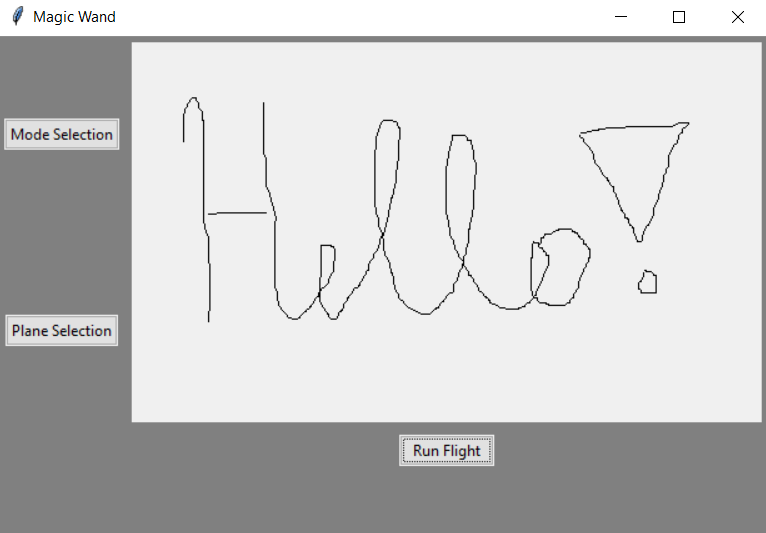
\includegraphics[width=0.75\textwidth]{docs/reports/Project Update 3/images/GUI.PNG}
        \caption{\textbf{GUI with allows for mouse drawing inputs.}}
        \label{fig:H_spectrum}
        \end{figure}

        As can be seen, there is a portion of the window reserved for drawing. Then the coordinates of this drawing are output. These coordinates are based on which pixel is being selected on the canvas. The buttons are configured to communicate to the drone. Currently, they output a message of choice when selected instead as a placeholder.
         
    \subsection{Week of November 8}
        
        The GUI will interface with an instance of the SimpleClient that will allow the user to execute flight through the interface. Through the defined canvas space, the pixel coordinates will be ported over to the SimpleClient instance where the coordinates will be translated to the real-world. Buttons will be implemented where the flight will follow the coordinates as shown in the canvas. 
        
        The GUI will also be refined in parallel. There will be specification for modes, incorporating for out future goals if encounter them. Radio buttons will also be implemented to specify the specific plane that the drone will follow the 2D path. These include the XY, XZ, and YZ planes that allow for the drone to fly in. Finally, a sub-interface will be utilized to save the flight data and other pertinent information that could be useful in understanding the flight. 
        
    \subsection{Week of November 15}
    With command and control via mouse and keyboard inputs demonstrated functionally, the DarwiinRemote program will interface with these systems as another input to remove the dependence on interacting via standard peripherals. The pairing of the remote with a macOS device will be attempted. Once successful, DarwiinRemote will be evaluated to ensure it functions as designed. If necessary, modifications to key/mouse binds within Tkinter will be made to ensure the Wii remote can replace standard inputs entirely while interacting with the drone.
    
    This will also require the implementation of infrared sources. The primary plan to do so involves purchasing infrared LEDs that can be powered via USB and clipped to the macOS device display. In theory, these sources could be placed anywhere in the room, though the clip method is judged as preferable for ease of pointing and intelligible drawing. If there are delays in the acquisition of infrared LEDs, candles or the official Wii sensor bar will be used.
    
    Throughout this process, the ergonomics of interacting with the drone will be evaluated. It is desirable to reduce the learning curve to interact in this way, so further refinements may be applied as they are identified.
    
    
    \subsection{Week of November 29}
    
     With the GUI fully functional, and a thorough interface provided between the DarwiinRemote, positional arguments, and CrazyFlie Client outputs, a majority of this projects goals have been completed. The methods above derived to loop in the Wii controller to interface with the client will be similarly used for these additional modes, and the group will allow the TA to complete a task objective for each additional mode by the week of November 29th.
    
    "Spellcaster" is where the group has drawn most of its inspiration, and provides the ethos for the drone controlled actions. Turning fantastical realms into reality is brought forth through this implementation, as the drone interprets user cast "spells" to perform certain objectives.
    
    In this way, the drone does not linearly move according to the direct coordinate input provided through the interface. Rather, in "Spellcaster" mode, a list of pre-determined Wii remote coordinate patterns will be matched with different movements to be completed by the drone. For example, as the user motions the Wii remote in a vertical line, the message is interpreted by the drone to lift and hover for a pre-defined amount of time.
    
    "Live" mode will then build off of the success of the first two mode implementations, "Copy Cat" and "Spellcaster". The goal of live mode is to interface between the Wii remote, code, and drone in real time. Positional arguments will be provided and interpreted by the drone while the user is using the remote, and it will position itself to align with the users remote movements. The overall goal is to enable a user experience similar to drawing. 
    
    Stretch goals deriving from this implementation are unbounded, and could include anything from a live, user controlled slow exposure light capture, to completion of a maze or other puzzles via user inputs to the drone. Additionally, the group would eventually like to include three-dimensional positional arguments, such that the drone could have the option to move into or out of a specified plane.
    
\section{Conclusion}
\textit{This section intentionally left blank.}

\newpage

\section*{Appendix}

    \appendix

\section{Group Member Contributions} \label{apx:contributions}
    \begin{table}[H]
        \begin{center}
        \setstretch{1}
        \caption{\textbf{Contributions Table}}
        \begin{tabular}{ | p{2in} | p{4in}| } 
            \hline
            \textbf{Group Member} & \textbf{Contribution to Project} \\  \hline
            Erika Jarosch & \\ \hline
            George Petrov & \\ \hline
            Justin Roskamp & \\ \hline
            Kenneth Tochihara & \\ \hline
        \end{tabular}
        \end{center}
    \end{table}

\section{Code Repository}
    GitHub Repository: \url{https://github.com/ktt3/ae483-magic-wand}


\section*{Acknowledgments}

    The authors thank their professor, Tim Bretl; their teaching assistant, Travis Zook; and their laboratory manager, Dan Block.
    
\bibliography{sample}

\end{document}